\chapter{Introduction}
\label{chap:intro}
\acresetall

This is an inline citation, \cite{braden2013}. This is a parenthetical citation \citep{braden2013}. This is a figure reference (Figure \ref{fig:footprint}). This is a section reference \S\ref{sec:intro:section_1}. This is a chapter reference with chapter spelled out: \autoref{chap:chapterI}. This is an acronym definition \ac{AGU}. This is the second time I use the acronym in this section \ac{AGU}. This is if I want to spell out the full acronym again \acf{AGU}. Define new acronyms in the acronyms.tex file.


%%%%%%%%%%%%%%%%%%%%%%%%%%%%%%%%%%%
\section{Section 1}
\label{sec:intro:section_1}
\lipsum[1] 

\begin{wrapfigure}{I}{0.5\textwidth}
\centering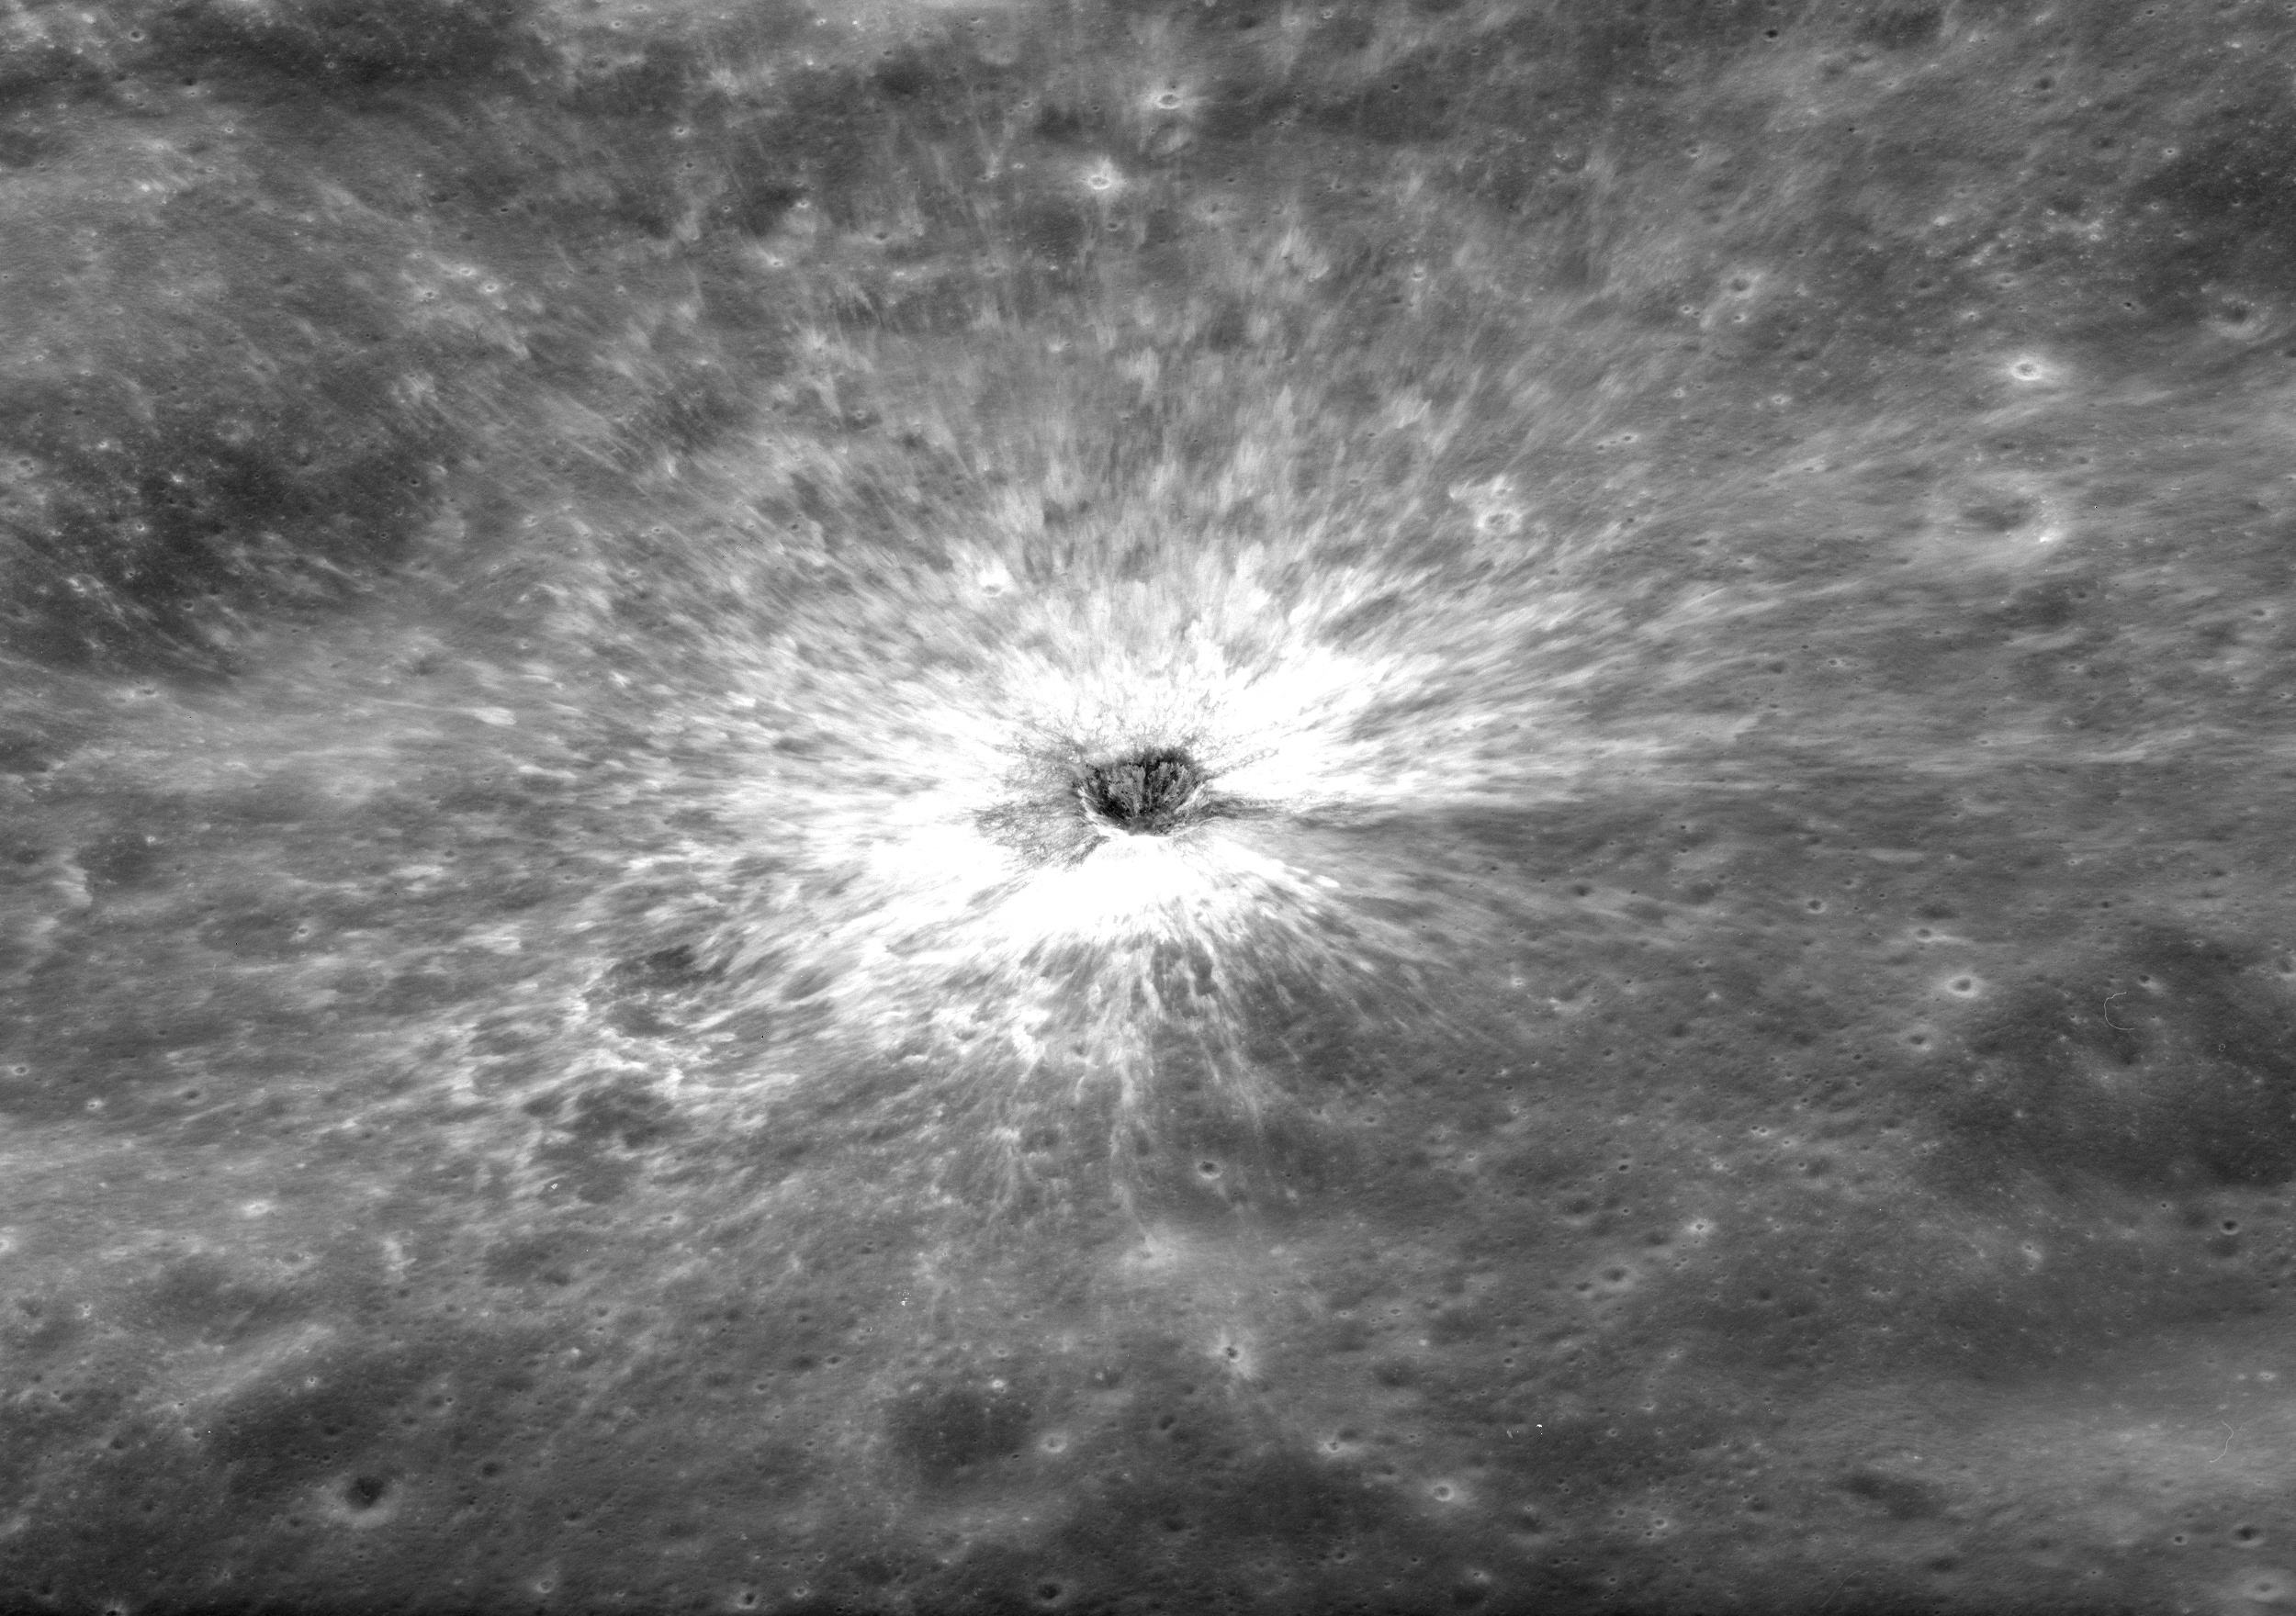
\includegraphics[width=\linewidth]{figs/chapter1/Bandfield_crater_AS17-P-2889.jpg}
\caption{Bandfield crater.}
\label{fig:footprint}
\end{wrapfigure}
\lipsum[1]
